%%%%%%%%%%%%%%%%%%%%%%%%%%%%%%%%%%%%%%%%%%%%%%%%%%%%%%%%%%%%%%%%%%%%%%%%%%%
\chapter{Include JSXGraph into web pages}
\label{ch:start}

\section{Additional files}
For including JSXGraph into HTML, two files are necessary:
\begin{itemize}
    \item jsxgraphcore.js
    \item jsxgraph.css
\end{itemize}
You can either download these two files and use the local copy or you can use the online version.
Then, the beginning of the HTML file should start like this:
\begin{fullwidth}\begin{lstlisting}[language=HTML]
<html>
<head>
 <link rel="stylesheet" type="text/css" href="jsxgraph.css" />
 <script type="text/javascript" src="jsxgraphcore.js"></script>
</head>
<body>
...
</body>
</html>
\end{lstlisting}\end{fullwidth}
If you want to include the online of JSXGraph in your HTML file then you have to write the following lines into the document head:
\begin{fullwidth}\begin{lstlisting}[language=HTML]
<html>
<head>
 <link rel="stylesheet" type="text/css" href="http://jsxgraph.uni-bayreuth.de/distrib/jsxgraph.css" />
 <script type="text/javascript" src="http://jsxgraph.uni-bayreuth.de/distrib/jsxgraphcore.js"></script>
</head>
<body>
...
</body>
</html>
\end{lstlisting}\end{fullwidth}

\section{The drawing panel}

The geometric construction which is displayed by JSXGraph resides in an HTML element. Usually, a div-element is taken. This division needs an ID. Using this ID, we declare this element to be a drawing panel of JSXGraph.

The following code has to be placed into the body part of an HTML file:
\begin{fullwidth}\begin{lstlisting}[language=HTML]
<div id="box" class="jxgbox"  style="width:500px; height:500px;"></div>
<script type="text/javascript"> 
 var board = JXG.JSXGraph.initBoard('box', {boundingbox:[-5,5,5,-5], axis:true});
</script>
\end{lstlisting}\end{fullwidth}
We can use as many different drawing panels as we like in one HTML file. The class jxgbox sets ``position:relative'' which seems to be mandatory for the Internet Explorer 7. 

Then, the web browser should display an element like the one shown in Figure~\ref{fig:1}.
\begin{figure*}[htb]
\centerline{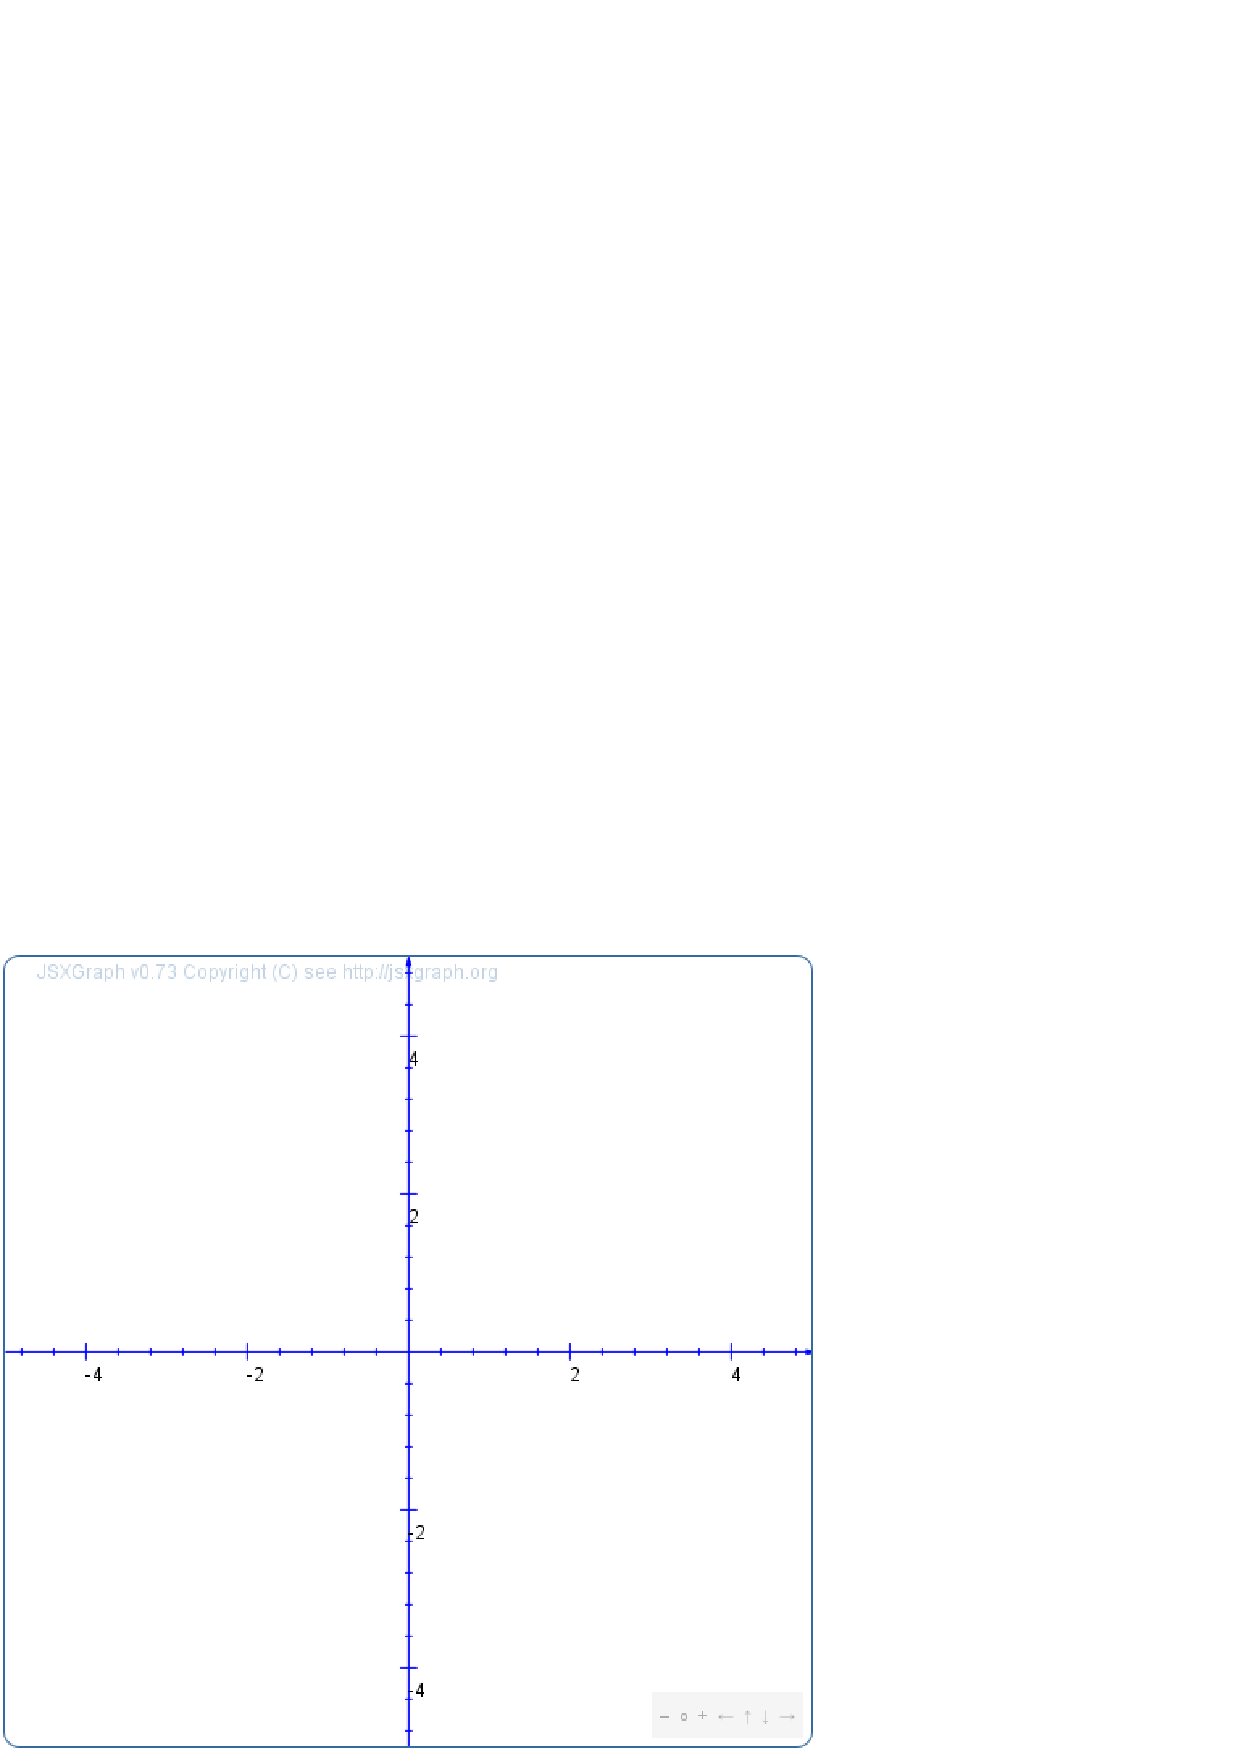
\includegraphics[width=0.4\linewidth]{images/b2.png}}
\caption{The first JSXGraph construction.}\label{fig:1}
\end{figure*}

The complete HTML file then looks like this:
\begin{fullwidth}\begin{lstlisting}[language=HTML]
<html>
<head>
 <link rel="stylesheet" type="text/css" href="jsxgraph.css" />
 <script type="text/javascript" src="jsxgraphcore.js"></script>
</head>
<body>
<div id="box" class="jxgbox" style="width:500px; height:500px;"></div>
<script type="text/javascript">
 var board = JXG.JSXGraph.initBoard('box', {boundingbox:[-5,5,5,-5], axis:true});
</script>
</body>
</html>
\end{lstlisting}\end{fullwidth}
Connect JSXGraph with the HTML div tag (usually at the end of the document body) and call 
the method \lstinline|initBoard()| of the global object \lstinline|JXG|

\begin{lstlisting}[language=HTML]
<script type="text/javascript">
 var board = JXG.JSXGraph.initBoard('box', 
            {boundingbox:[-5,5,5,-5], axis:true});
</script>
\end{lstlisting}
The method \lstinline|initBoard()| may have two arguments:
\begin{itemize}
    \item Parameter 1: the \lstinline|id| of the div tag in the HTML page which will contain the JSXGraph construction.
    \item (optional) Parameter 2: additional properties of the board. 
\end{itemize}
The possible optional properties of the board are:

    * originX, originY (in pixel)
    * unitX, unitY (in pixel)
    * zoomX, zoomY
    * Bounding box
    * axis (true/false)
    * grid (true/false)
    * showNavigation (true/false)
    * showCopyright (true/false) 

More than one boards can be initialised simultaneously in one HTML file. 
